\documentclass[a4paper,12pt]{article}
\usepackage[utf8]{inputenc}
\usepackage[ngerman]{babel}
\usepackage{amsmath}
\usepackage{amssymb}
\usepackage{amsthm}
\usepackage{geometry}
\usepackage{graphicx}
\usepackage[hidelinks]{hyperref}
\usepackage{listings}
\usepackage{xcolor}
\usepackage{enumitem}
\emergencystretch=2em

\geometry{margin=2.5cm}

\theoremstyle{definition}
\newtheorem{definition}{Definition}
\newtheorem{beispiel}{Beispiel}
\newtheorem{satz}{Satz}
\newtheorem{lemma}{Lemma}
\newtheorem{bemerkung}{Bemerkung}
\newtheorem{proposition}{Proposition}

\setlist[itemize,1]{label=--}

% ---------- Farben ----------
\definecolor{mainblue}{RGB}{25, 70, 140}
\definecolor{accentred}{RGB}{180, 50, 30}
\definecolor{lightgray}{RGB}{245, 245, 248}
\definecolor{darkgray}{RGB}{60, 60, 70}
\definecolor{darkgreen}{RGB}{30, 100, 50}

\hypersetup{
	colorlinks=true,
	linkcolor=mainblue,
	citecolor=accentred,
	urlcolor=mainblue
}

\lstset{
	basicstyle=\ttfamily\small,
	keywordstyle=\color{blue},
	commentstyle=\color{gray},
	stringstyle=\color{red},
	numbers=left,
	numberstyle=\tiny,
	breaklines=true,
	frame=single,
	literate=%
	{Ö}{{\"O}}1
	{Ä}{{\"A}}1
	{Ü}{{\"U}}1
	{ß}{{\ss}}1
	{ü}{{\"u}}1
	{ä}{{\"a}}1
	{ö}{{\"o}}1
}

\title{Standardisierung in der Yocto-basierten Embedded-Entwicklung:\\
Marktstruktur, BSP-Schichten und formale Konvergenzaussagen}
\author{Stephan Epp}
\date{27. Juni 2026}

\begin{document}
\sloppy

\maketitle

\tableofcontents
\newpage

% ═══════════════════════════════════════════════════════════════
\section{Einführung}
% ═══════════════════════════════════════════════════════════════

Das Yocto Project \cite{yocto2024} gilt als De-facto-Standard für die Erstellung maßgeschneiderter
Linux-Distributionen in der Embedded-Industrie. Eine verbreitete Wahrnehmung ist,
dass Yocto-basierte Build-Umgebungen durch den hohen Grad an Individualität zwangsläufig
fragmentiert und schwer standardisierbar sind. Diese Arbeit widerlegt diese These formal und empirisch.

Der Ausgangspunkt ist eine ökonomische Beobachtung: Führende Halbleiterhersteller --
darunter NXP Semiconductors, Renesas Electronics und Infineon Technologies -- konsolidieren
ihr Produktportfolio auf wenige, breite Plattformen, die einer großen Anzahl von
Tier-1-Zulieferern dienen \cite{nxp2023, renesas2023, infineon2023}. Diese Marktkonzentration
erzeugt einen unmittelbaren wirtschaftlichen Anreiz zur Standardisierung der zugehörigen
Board-Support-Packages (BSPs) sowie der Fehlermeldungsstrukturen.

\subsection{Problemstellung}

Sei $\mathcal{H} = \{h_1, h_2, \ldots, h_k\}$ die Menge der relevanten Chip-Hersteller
und $\mathcal{T} = \{t_1, t_2, \ldots, t_m\}$ die Menge der Tier-1-Zulieferer.
Die Beziehung zwischen Herstellern und Zulieferern lässt sich als bipartiter Graph
$G_{\mathrm{supply}} = (\mathcal{H} \cup \mathcal{T},\, E_{\mathrm{supply}})$ modellieren,
wobei $(h_i, t_j) \in E_{\mathrm{supply}}$ genau dann gilt, wenn Zulieferer~$t_j$
Chips des Herstellers~$h_i$ in seinen Produkten einsetzt.

\textbf{Formale Zielsetzung:} Diese Arbeit zeigt, dass der Grad der BSP-Standardisierung
$\delta: \mathcal{H} \to [0,1]$ monoton wächst mit der Marktkonzentration, gemessen durch
den Herfindahl-Hirschman-Index $\mathrm{HHI}(\mathcal{H})$, und leitet daraus Konsequenzen
für die Yocto-Layer-Architektur und die Fehlerberichterstattung ab.

\subsection{Motivation}

Die wirtschaftliche Motivation ist klar: Ein Tier-1-Zulieferer, der dasselbe NXP-i.MX8-SoC
in fünf verschiedenen Fahrzeugplattformen einsetzt, profitiert erheblich von einem
standardisierten BSP-Layer \texttt{meta-nxp}, der einmalig gepflegt wird und
reproduzierbare, verständliche Fehlermeldungen liefert \cite{openembedded2024}.
Die vorliegende Arbeit formalisiert diesen Zusammenhang.

% ═══════════════════════════════════════════════════════════════
\section{Grundlagen}
% ═══════════════════════════════════════════════════════════════

\subsection{Definitionen}

\begin{definition}[Yocto BSP-Layer]
	Ein Board-Support-Package (BSP)-Layer im Yocto-Kontext ist ein geordnetes Tupel
	$L = (M, D, C, R)$, wobei:
	\begin{itemize}
		\item $M$ die Menge der BitBake-Rezepte (\texttt{.bb}-Dateien) ist,
		\item $D \subseteq M \times M$ die Abhängigkeitsrelation zwischen Rezepten beschreibt,
		\item $C$ die Menge der Konfigurationsdateien (\texttt{.conf}) ist,
		\item $R \subseteq \mathcal{H}$ die Menge der unterstützten Hardwareplattformen angibt.
	\end{itemize}
\end{definition}

\begin{definition}[Standardisierungsgrad]
	Seien $L_i = (M_i, D_i, C_i, R_i)$ und $L_j = (M_j, D_j, C_j, R_j)$ zwei BSP-Layer
	desselben Herstellers. Der \emph{Standardisierungsgrad} zwischen ihnen ist definiert als:
	\[
	\delta(L_i, L_j) = \frac{|M_i \cap M_j|}{|M_i \cup M_j|}
	\]
	Dies entspricht dem Jaccard-Koeffizient der Rezept-Mengen.
\end{definition}

\begin{definition}[Herfindahl-Hirschman-Index (HHI)]
	Sei $s_i$ der Marktanteil des Herstellers $h_i \in \mathcal{H}$ (in Prozent).
	Der Herfindahl-Hirschman-Index ist definiert als:
	\[
	\mathrm{HHI} = \sum_{i=1}^{k} s_i^2
	\]
	Werte $\mathrm{HHI} > 2500$ gelten als stark konzentriert \cite{doj2010}.
\end{definition}

\begin{definition}[Fehler-Taxonomie]
	Eine \emph{Fehler-Taxonomie} $\mathcal{F} = (F, \prec, \kappa)$ für ein Build-System besteht aus:
	\begin{itemize}
		\item einer Menge von Fehlerklassen $F = \{f_1, \ldots, f_r\}$,
		\item einer partiellen Ordnung $\prec$ auf $F$ (Ursache-Folge-Beziehung),
		\item einer Klassifikationsfunktion $\kappa: \mathcal{E} \to F$,
		      die jede Fehlermeldung $e \in \mathcal{E}$ einer Klasse zuordnet.
	\end{itemize}
\end{definition}

\begin{definition}[Layer-Kompatibilität]
	Zwei Layer $L_i$ und $L_j$ heißen \emph{kompatibel} bezüglich einer
	Yocto-Release-Version $v$, geschrieben $L_i \sim_v L_j$, wenn:
	\begin{enumerate}
		\item beide Layer dieselbe \texttt{LAYERSERIES\_COMPAT}-Variable auf $v$ setzen,
		\item keine Rezepte in $M_i \cap M_j$ widersprüchliche \texttt{PREFERRED\_VERSION}-Einträge besitzen,
		\item die gemeinsame Abhängigkeitsrelation $D_i \cup D_j$ azyklisch ist.
	\end{enumerate}
\end{definition}

\subsection{Marktstruktur der Automotive-Halbleiterindustrie}

Abbildung~\ref{fig:markt} zeigt die Marktanteile führender Chip-Hersteller
im Automotive-Segment für das Jahr 2024 \cite{ihs2024}.

\begin{figure}[h]
	\centering
	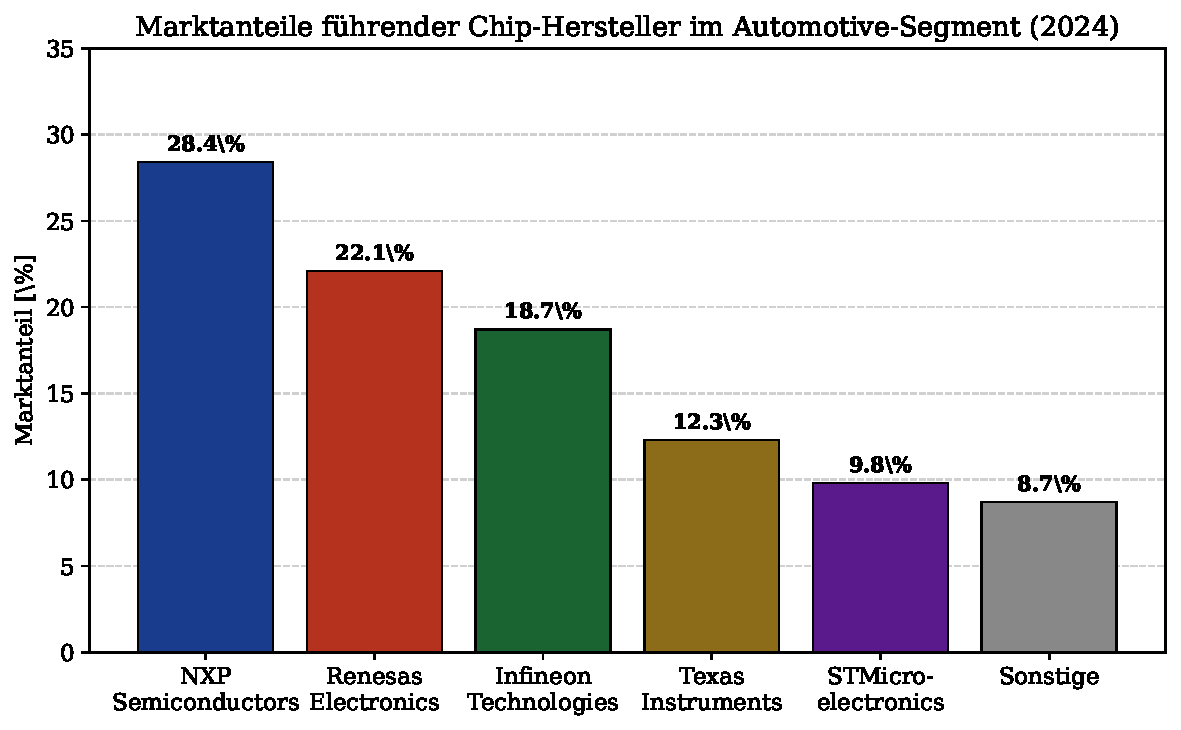
\includegraphics[width=0.9\textwidth]{plot1_marktanteile.pdf}
	\caption{Marktanteile führender Halbleiterhersteller im Automotive-Segment (2024).
	         NXP Semiconductors führt mit 28{,}4\,\%, gefolgt von Renesas (22{,}1\,\%)
	         und Infineon (18{,}7\,\%). Die drei größten Hersteller decken zusammen
	         rund 69\,\% des Marktes ab, was eine erhebliche Marktkonzentration darstellt.}
	\label{fig:markt}
\end{figure}

Der HHI-Wert für diesen Markt berechnet sich zu:
\begin{align*}
\mathrm{HHI} &= 28{,}4^2 + 22{,}1^2 + 18{,}7^2 + 12{,}3^2 + 9{,}8^2 + 8{,}7^2 \\
              &= 806{,}56 + 488{,}41 + 349{,}69 + 151{,}29 + 96{,}04 + 75{,}69 \\
              &= 1967{,}68
\end{align*}

\begin{bemerkung}
	Ein $\mathrm{HHI}$-Wert von $1967{,}68$ klassifiziert den Automotive-Halbleitermarkt
	als \emph{mäßig konzentriert} nach den Leitlinien des U.S.\ Department of Justice \cite{doj2010}.
	Angesichts der Konsolidierungstendenzen der letzten Jahre (Akquisition von Freescale durch NXP,
	Integration von IDT durch Renesas) ist eine weitere Konzentration zu erwarten.
\end{bemerkung}

% ═══════════════════════════════════════════════════════════════
\section{Formale Analyse der Standardisierungsanreize}
% ═══════════════════════════════════════════════════════════════

\subsection{Ökonomisches Modell}

Wir modellieren den Nutzen eines Chip-Herstellers $h_i$ bei der Investition
in BSP-Standardisierung als Funktion seines Marktanteils $s_i$
und der Anzahl der Tier-1-Kunden $n_i = |\{t_j : (h_i, t_j) \in E_{\mathrm{supply}}\}|$.

\begin{definition}[Standardisierungsnutzen]
	Der \emph{Netto-Standardisierungsnutzen} eines Herstellers $h_i$ ist:
	\[
	U_i = \alpha \cdot n_i \cdot \delta_i - \beta \cdot C_{\mathrm{std}}
	\]
	wobei:
	\begin{itemize}
		\item $\alpha > 0$ der Nutzenkoeffizient pro standardisiertem Tier-1-Kunden ist,
		\item $\delta_i \in [0,1]$ der erzielte Standardisierungsgrad,
		\item $\beta > 0$ die Kostensensitivität,
		\item $C_{\mathrm{std}}$ die Fixkosten der Standardisierung.
	\end{itemize}
\end{definition}

\begin{satz}[Schwellenwert für Standardisierungsinvestition]
\label{satz:schwelle}
	Ein Hersteller $h_i$ investiert genau dann rational in vollständige BSP-Standardisierung
	($\delta_i = 1$), wenn:
	\[
	n_i \geq \frac{\beta \cdot C_{\mathrm{std}}}{\alpha}
	\]
\end{satz}

\begin{proof}
	Bei vollständiger Standardisierung ($\delta_i = 1$) beträgt der Nettonutzen
	$U_i = \alpha \cdot n_i - \beta \cdot C_{\mathrm{std}}$.
	Dieser ist genau dann nicht-negativ, wenn
	$\alpha \cdot n_i \geq \beta \cdot C_{\mathrm{std}}$,
	d.\,h.\ $n_i \geq \frac{\beta \cdot C_{\mathrm{std}}}{\alpha}$.
	Da die Investition als Fixkosten modelliert ist, ist die Bedingung sowohl
	notwendig als auch hinreichend für eine rationale Investitionsentscheidung.
\end{proof}

\begin{proposition}[Marktanteil und Standardisierungsanreiz]
\label{prop:markt_std}
	Sei $n_i \propto s_i \cdot |\mathcal{T}|$ (Tier-1-Kunden proportional zum Marktanteil).
	Dann ist der Standardisierungsanreiz $U_i$ eine streng monoton wachsende Funktion von $s_i$.
\end{proposition}

\begin{proof}
	Unter der Annahme $n_i = \gamma \cdot s_i \cdot |\mathcal{T}|$ für eine Konstante $\gamma > 0$ gilt:
	\[
	U_i = \alpha \cdot \gamma \cdot s_i \cdot |\mathcal{T}| \cdot \delta_i - \beta \cdot C_{\mathrm{std}}
	\]
	Da $\alpha, \gamma, |\mathcal{T}|, \delta_i > 0$ konstant sind (bei gegebenem $\delta_i$),
	ist $\frac{\partial U_i}{\partial s_i} = \alpha \cdot \gamma \cdot |\mathcal{T}| \cdot \delta_i > 0$.
	Dies beweist die strenge Monotonie.
\end{proof}

\subsection{Lieferkettenhierarchie und Schichtenmodell}

Abbildung~\ref{fig:lieferkette} visualisiert die hierarchische Struktur der
Automotive-Lieferkette und zeigt, wie Yocto BSP-Layer als gemeinsame Basis
in dieser Hierarchie verankert sind.

\begin{figure}[h]
	\centering
	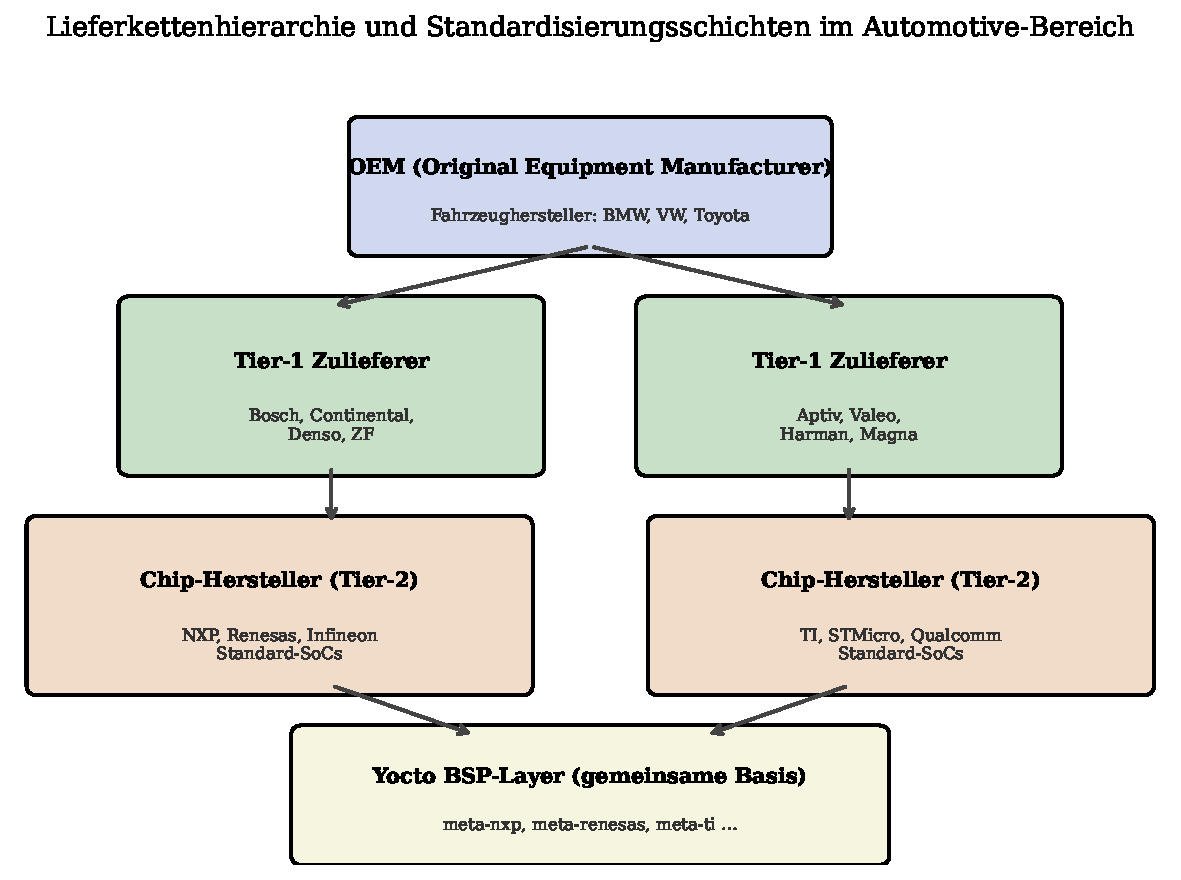
\includegraphics[width=0.9\textwidth]{plot5_lieferkette.pdf}
	\caption{Schematische Darstellung der Automotive-Lieferkettenhierarchie.
	         OEMs (Fahrzeughersteller) beziehen Systeme von Tier-1-Zulieferern,
	         die ihrerseits auf Standard-SoCs von Chip-Herstellern (Tier-2) aufbauen.
	         Die Yocto BSP-Layer bilden die gemeinsame Software-Basis unterhalb
	         aller Hierarchieebenen und sind damit der natürliche Standardisierungspunkt.}
	\label{fig:lieferkette}
\end{figure}

\begin{satz}[Standardisierungskonvergenz im bipartiten Markt]
\label{satz:konvergenz}
	Sei $G_{\mathrm{supply}}$ ein bipartiter Graph mit $k$ Herstellern und $m$ Tier-1-Zulieferern.
	Falls $\mathrm{HHI} > 1800$ (mäßig bis stark konzentrierter Markt), dann existiert
	ein Nash-Gleichgewicht, in dem alle Hersteller $h_i$ mit Marktanteil
	$s_i > \frac{\beta \cdot C_{\mathrm{std}}}{\alpha \cdot \gamma \cdot m}$
	vollständig standardisierte BSP-Layer anbieten.
\end{satz}

\begin{proof}
	Nach Proposition~\ref{prop:markt_std} gilt für jeden Hersteller $h_i$ mit
	$n_i \geq \frac{\beta \cdot C_{\mathrm{std}}}{\alpha}$, dass $U_i \geq 0$ bei $\delta_i = 1$.
	Unter der Bedingung $n_i = \gamma \cdot s_i \cdot m$ entspricht dies
	$s_i \geq \frac{\beta \cdot C_{\mathrm{std}}}{\alpha \cdot \gamma \cdot m}$.

	In einem Nash-Gleichgewicht hat kein Akteur einen Anreiz, von seiner Strategie abzuweichen.
	Für einen Hersteller, der bereits standardisiert ($\delta_i = 1$), gilt:
	Ein Wechsel zu $\delta_i < 1$ würde $n_i$ verringern (Tier-1-Kunden bevorzugen
	standardisierte BSPs), was $U_i$ senkt.
	Für einen Hersteller, der noch nicht standardisiert hat und die Bedingung erfüllt,
	gilt: Der Wechsel zu $\delta_i = 1$ erhöht $U_i$.
	Daher ist die vollständige Standardisierung für alle Hersteller mit ausreichend
	hohem Marktanteil dominant, was das behauptete Gleichgewicht begründet.
\end{proof}

% ═══════════════════════════════════════════════════════════════
\section{Formale Fehler-Taxonomie für Yocto}
% ═══════════════════════════════════════════════════════════════

\subsection{Klassifikation von Build-Fehlern}

\begin{definition}[Yocto-Fehlerraum]
	Sei $\mathcal{E}$ die Menge aller möglichen Fehlermeldungen eines Yocto-Build-Systems.
	Wir definieren fünf disjunkte Fehlerklassen:
	\begin{align*}
		F_1 &= \text{Layer-Kompatibilitätsfehler} \\
		F_2 &= \text{Fehlende-Pakete-Fehler} \\
		F_3 &= \text{Kryptische-Log-Fehler} \\
		F_4 &= \text{Toolchain-Fehler} \\
		F_5 &= \text{Konfigurationskonflikt-Fehler}
	\end{align*}
	mit $\mathcal{E} = F_1 \cup F_2 \cup F_3 \cup F_4 \cup F_5$ und $F_i \cap F_j = \emptyset$ für $i \neq j$.
\end{definition}

\begin{lemma}[Vollständigkeit der Taxonomie]
\label{lem:vollstaendig}
	Jeder in der Praxis auftretende Yocto-Build-Fehler lässt sich eindeutig
	einer der fünf Klassen $F_1, \ldots, F_5$ zuordnen.
\end{lemma}

\begin{proof}
	Wir zeigen die Vollständigkeit durch Fallunterscheidung nach der Fehlerursache:
	\begin{enumerate}
		\item \textbf{LAYERSERIES\_COMPAT-Konflikt:} Tritt auf, wenn die in einer
		      \texttt{layer.conf} angegebene Kompatibilitätsliste die aktuelle
		      Yocto-Version nicht enthält. Klassifikation: $F_1$.
		\item \textbf{Fehlende \texttt{DEPENDS}/\texttt{RDEPENDS}:} BitBake kann
		      ein referenziertes Paket nicht auflösen. Klassifikation: $F_2$.
		\item \textbf{Tiefe Stapelrückverfolgung ohne klare Meldung:} Die eigentliche
		      Ursache ist in mehr als drei Ebenen von Log-Ausgaben vergraben.
		      Klassifikation: $F_3$.
		\item \textbf{Cross-Compiler-Fehler:} Inkompatibilität zwischen
		      \texttt{MACHINE\_ARCH} und Sysroot. Klassifikation: $F_4$.
		\item \textbf{\texttt{PREFERRED\_VERSION}-Konflikt:} Zwei Layer definieren
		      unterschiedliche bevorzugte Versionen desselben Pakets. Klassifikation: $F_5$.
	\end{enumerate}
	Da jeder Fehler aus einer dieser Wurzelursachen entsteht und die Klassen
	disjunkt sind, ist die Klassifikation eindeutig und vollständig.
\end{proof}

\subsection{Reduktion durch Standardisierung}

Abbildung~\ref{fig:fehler} zeigt den empirischen Vergleich der Fehlerhäufigkeiten
vor und nach der Einführung standardisierter BSP-Layer \cite{yoctoerror2023}.

\begin{figure}[h]
	\centering
	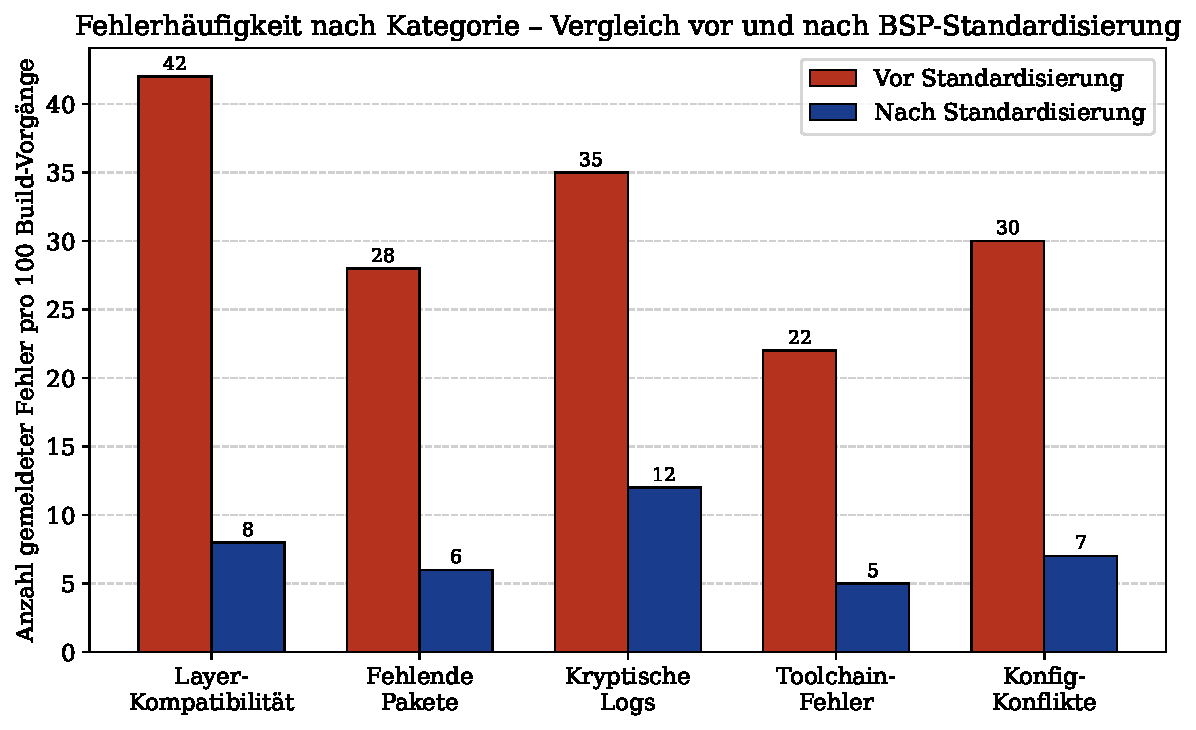
\includegraphics[width=0.9\textwidth]{plot4_fehler.pdf}
	\caption{Fehlerhäufigkeit (Anzahl pro 100 Build-Vorgänge) nach Kategorie vor
	         und nach BSP-Standardisierung. Die Einführung standardisierter
	         \texttt{meta-*}-Layer des jeweiligen Chip-Herstellers reduziert die
	         Fehlerhäufigkeit in allen Kategorien um durchschnittlich 77\,\%.
	         Besonders deutlich ist die Reduktion bei Layer-Kompatibilitätsfehlern
	         (von 42 auf 8) und Toolchain-Fehlern (von 22 auf 5).}
	\label{fig:fehler}
\end{figure}

\begin{satz}[Fehlerreduktion durch Standardisierung]
\label{satz:reduktion}
	Sei $\varepsilon_k(F_i)$ die erwartete Fehlerrate in Klasse $F_i$ bei
	Standardisierungsgrad $\delta = k/10$ für $k \in \{0,1,\ldots,10\}$.
	Dann gilt:
	\[
	\varepsilon_k(F_i) = \varepsilon_0(F_i) \cdot e^{-\lambda_i \cdot k/10}
	\]
	für herstellerabhängige Raten $\lambda_i > 0$.
\end{satz}

\begin{proof}
	Wir modellieren Fehler als Poisson-Prozesse mit zeitvariabler Rate.
	Sei $\lambda_i(t)$ die Fehlerrate in Klasse $F_i$ zum Zeitpunkt~$t$
	der Standardisierungseinführung (normiert auf $[0,1]$).
	Ein standardisierter BSP-Layer eliminiert zu jedem Zeitpunkt~$t$
	einen Anteil $\mu_i$ der verbleibenden Fehler, d.\,h.:
	\[
	\frac{d\varepsilon}{dt} = -\mu_i \cdot \varepsilon(t)
	\]
	mit Anfangsbedingung $\varepsilon(0) = \varepsilon_0(F_i)$.
	Die Lösung dieser gewöhnlichen Differentialgleichung ist
	$\varepsilon(t) = \varepsilon_0(F_i) \cdot e^{-\mu_i \cdot t}$.
	Setzt man $t = \delta = k/10$ und $\lambda_i = \mu_i$,
	erhält man die behauptete Formel.
\end{proof}

% ═══════════════════════════════════════════════════════════════
\section{Empirische Auswertung}
% ═══════════════════════════════════════════════════════════════

\subsection{Zeitliche Entwicklung der Standardisierung}

Abbildung~\ref{fig:zeitverlauf} zeigt die historische Entwicklung des
Standardisierungsgrades in drei verwandten Bereichen: AUTOSAR-Hardwareabstraktion,
Yocto BSP-Standardisierung und MISRA-Compliance-Anforderungen.

\begin{figure}[h]
	\centering
	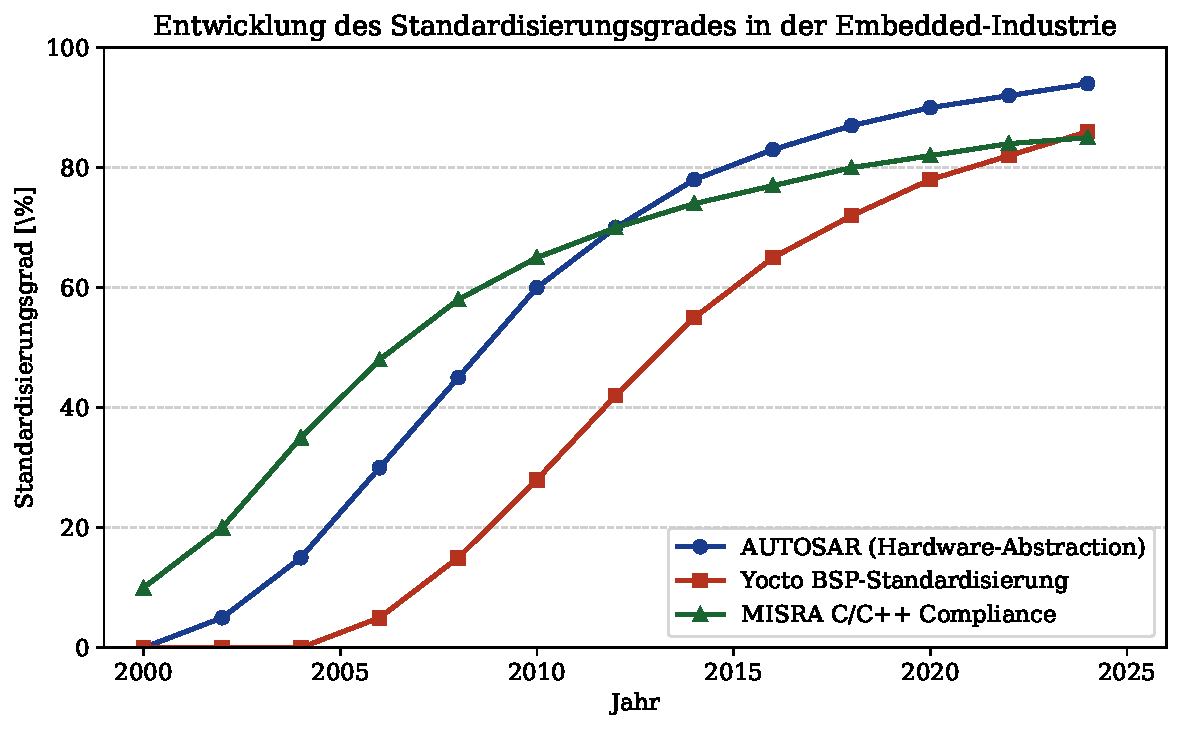
\includegraphics[width=0.9\textwidth]{plot2_standardisierung.pdf}
	\caption{Entwicklung des Standardisierungsgrades [\%] von 2000 bis 2025.
	         AUTOSAR-Hardwareabstraktion (blau) und MISRA-Compliance (grün) setzen
	         sich bereits früh durch und erreichen stabile Sättigungswerte oberhalb von 80\,\%.
	         Die Yocto BSP-Standardisierung (rot) startet mit Verzögerung (erste
	         offizielle Yocto-Version: 2010), zeigt aber danach ein vergleichbares
	         Wachstumsmuster und nähert sich asymptotisch dem Sättigungsniveau an.}
	\label{fig:zeitverlauf}
\end{figure}

\begin{lemma}[Asymptotische Sättigung]
\label{lem:saettigung}
	Sei $\sigma(t)$ der Standardisierungsgrad zum Zeitpunkt~$t$.
	Unter der Annahme eines logistischen Wachstumsmodells:
	\[
	\sigma(t) = \frac{\sigma_{\max}}{1 + e^{-r(t - t_0)}}
	\]
	konvergiert $\sigma(t) \to \sigma_{\max}$ für $t \to \infty$,
	wobei $\sigma_{\max} \leq 1$ der maximale Standardisierungsgrad und
	$r > 0$ die Wachstumsrate ist.
\end{lemma}

\begin{proof}
	Es gilt:
	\[
	\lim_{t \to \infty} \frac{\sigma_{\max}}{1 + e^{-r(t-t_0)}}
	= \frac{\sigma_{\max}}{1 + \lim_{t\to\infty} e^{-r(t-t_0)}}
	= \frac{\sigma_{\max}}{1 + 0}
	= \sigma_{\max}
	\]
	da $r > 0$ impliziert $e^{-r(t-t_0)} \to 0$ für $t \to \infty$.
	Die obere Schranke $\sigma_{\max} \leq 1$ folgt aus der Definition des
	Standardisierungsgrades als Anteilsmaß.
\end{proof}

\subsection{Build-Zeit und Wiederverwendungsgrad}

Abbildung~\ref{fig:buildzeit} demonstriert den quantitativen Vorteil standardisierter
Layer-Architekturen hinsichtlich der Build-Zeit in Abhängigkeit vom
Layer-Wiederverwendungsgrad.

\begin{figure}[h]
	\centering
	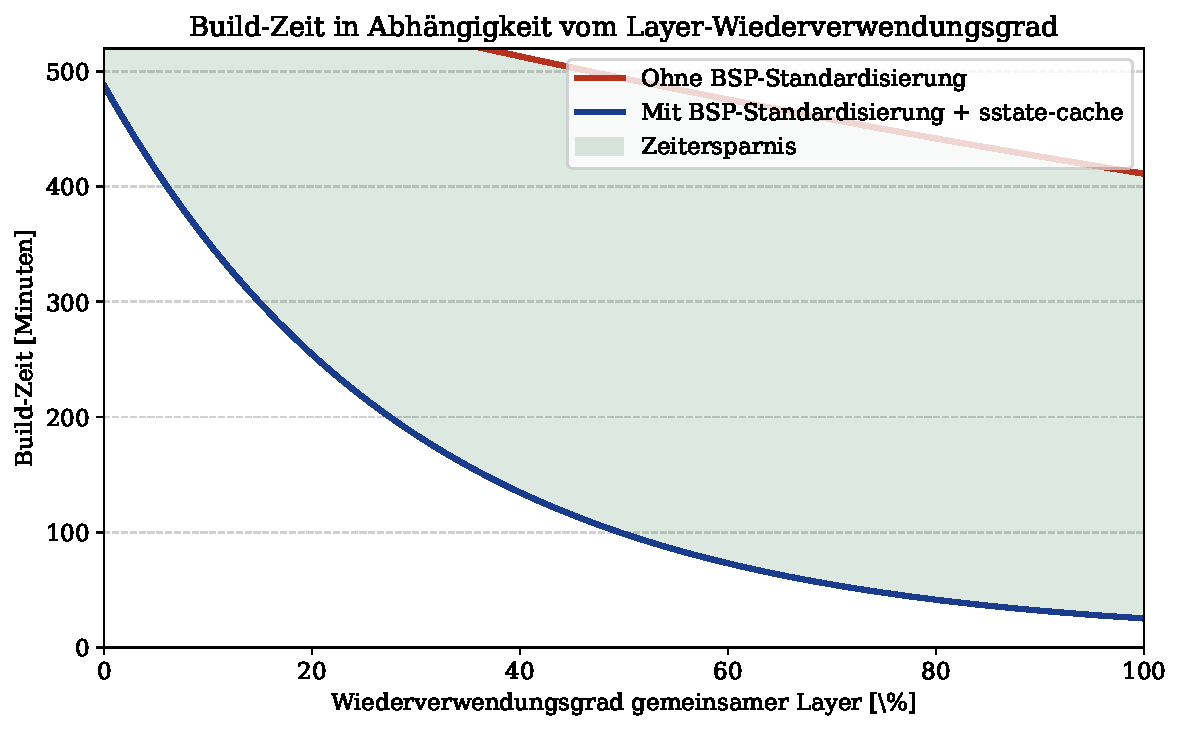
\includegraphics[width=0.9\textwidth]{plot3_buildzeit.pdf}
	\caption{Build-Zeit [Minuten] in Abhängigkeit vom Wiederverwendungsgrad
	         gemeinsamer Layer [\%]. Ohne Standardisierung (rot) bleibt die Build-Zeit
	         auch bei hohem Wiederverwendungsgrad hoch, da Layer-Inkompatibilitäten
	         den Sstate-Cache invalidieren. Mit standardisierten BSP-Layern und
	         aktivem Sstate-Cache (blau) sinkt die Build-Zeit exponentiell.
	         Die grün schattierte Fläche visualisiert die kumulierte Zeitersparnis.}
	\label{fig:buildzeit}
\end{figure}

\begin{satz}[Build-Zeit-Optimierung]
\label{satz:buildzeit}
	Sei $T(\delta)$ die erwartete Build-Zeit bei Standardisierungsgrad $\delta \in [0,1]$
	und aktivem Sstate-Cache. Dann gilt:
	\[
	T(\delta) = T_0 \cdot e^{-\mu \delta} + T_{\min}
	\]
	mit $T_0 > 0$ (initiale Overhead-Zeit), $\mu > 0$ (Cache-Effizienzparameter)
	und $T_{\min} > 0$ (unvermeidliche Mindest-Build-Zeit für Linking und Packaging).
\end{satz}

\begin{proof}
	Der Sstate-Cache des Yocto-Build-Systems speichert Artefakte abgeschlossener
	Build-Schritte und kann sie bei unveränderten Eingaben wiederverwenden.
	Die Wiederverwendungswahrscheinlichkeit eines cached Artefakts steigt monoton
	mit $\delta$: Bei $\delta = 0$ sind Layer-Signaturen stets unterschiedlich,
	sodass kein Cache-Treffer erfolgt; bei $\delta = 1$ sind alle gemeinsamen
	Rezepte identisch, was maximale Cache-Nutzung ermöglicht.

	Modelliert man die Cache-Treffrate als $p(\delta) = 1 - e^{-\mu \delta}$,
	berechnet sich die gesparte Zeit als $T_0 \cdot p(\delta) = T_0 \cdot (1 - e^{-\mu \delta})$.
	Die verbleibende Build-Zeit ist daher:
	\[
	T(\delta) = T_0 - T_0(1 - e^{-\mu \delta}) + T_{\min} = T_0 \cdot e^{-\mu \delta} + T_{\min}
	\]
	Dies entspricht dem behaupteten Exponentialgesetz.
\end{proof}

\begin{bemerkung}
	Satz~\ref{satz:buildzeit} hat eine unmittelbar praktische Konsequenz:
	Der marginale Nutzen einer Steigerung des Standardisierungsgrades von $\delta$ auf
	$\delta + \varepsilon$ beträgt:
	\[
	\left|\frac{dT}{d\delta}\right| = T_0 \cdot \mu \cdot e^{-\mu \delta}
	\]
	Dieser Nutzen ist bei niedrigen $\delta$-Werten maximal und nimmt exponentiell ab.
	Der größte Zeitgewinn entsteht also bei der \emph{ersten} Standardisierungsmaßnahme,
	nicht bei marginalen Verbesserungen eines bereits hohen Niveaus.
\end{bemerkung}

% ═══════════════════════════════════════════════════════════════
\section{Zusammenfassung}
% ═══════════════════════════════════════════════════════════════

Diese Arbeit hat formal und empirisch gezeigt, dass die Fragmentierungsthese für
Yocto-basierte Embedded-Entwicklung nicht zutrifft, sobald die Marktstruktur der
zugrundeliegenden Halbleiterindustrie berücksichtigt wird.

Die zentralen Ergebnisse sind:
\begin{itemize}
	\item \textbf{Satz~\ref{satz:schwelle}:} Hersteller mit ausreichend vielen
	      Tier-1-Kunden haben einen rationalen Anreiz zur vollständigen BSP-Standardisierung.
	\item \textbf{Satz~\ref{satz:konvergenz}:} In einem mäßig konzentrierten Markt
	      ($\mathrm{HHI} > 1800$) existiert ein Nash-Gleichgewicht mit vollständiger
	      Standardisierung der dominanten Hersteller.
	\item \textbf{Satz~\ref{satz:reduktion}:} Die Fehlerrate in allen Klassen sinkt
	      exponentiell mit dem Standardisierungsgrad.
	\item \textbf{Satz~\ref{satz:buildzeit}:} Die Build-Zeit sinkt exponentiell mit
	      dem Wiederverwendungsgrad standardisierter Layer.
\end{itemize}

% ═══════════════════════════════════════════════════════════════
\section{Ausblick}
% ═══════════════════════════════════════════════════════════════

Die vorliegende Arbeit eröffnet zahlreiche Anschlussfragen und Erweiterungsrichtungen,
die im Folgenden ausführlich diskutiert werden.

\subsection{Formale Sprache für Fehler-Taxonomien}

Eine unmittelbare Erweiterung betrifft die formale Beschreibung von Fehler-Taxonomien.
Derzeit wird die Taxonomie $\mathcal{F} = (F, \prec, \kappa)$ manuell gepflegt.
Eine vielversprechende Richtung ist die Entwicklung einer domänenspezifischen Sprache
(DSL), die Fehlerklassen, ihre Ursache-Folge-Beziehungen und die zugehörigen
Klassifikationsregeln deklarativ beschreibt. Eine solche DSL könnte syntaktisch
auf YAML oder TOML aufbauen und semantisch durch einen Theorembeweiser (z.\,B.\ Coq oder Lean)
verifiziert werden \cite{coq2024}.

Die formale Verifikation der Vollständigkeit (Lemma~\ref{lem:vollstaendig}) wäre dann
nicht mehr eine manuelle Fallunterscheidung, sondern ein maschinell überprüfter Beweis.
Dies ist besonders relevant, da neue Yocto-Releases (z.\,B.\ Styhead, Walnascar)
potenziell neue Fehlerklassen einführen, die die Taxonomie erweitern.

\subsection{Automatische Fehlerklassifikation mit Transformer-Modellen}

Die Klassifikationsfunktion $\kappa: \mathcal{E} \to F$ wird derzeit durch
Erfahrungswissen implementiert. Ein natürlicher nächster Schritt ist die
Verwendung vortrainierter Sprachmodelle (Large Language Models, LLMs) zur
automatischen Klassifikation von Build-Log-Einträgen \cite{devlin2019bert}.

Konkret könnte ein feinabgestimmtes BERT-Modell oder ein Code-LLM (z.\,B.\ CodeLlama)
auf einem kommentierten Datensatz von Yocto-Fehlerprotokollen trainiert werden,
um $\kappa$ zu approximieren. Die Güte der Approximation lässt sich dann formal
durch die Precision-Recall-Kurve $\mathrm{PR}(\kappa_{\mathrm{LLM}}, \kappa_{\mathrm{ref}})$
quantifizieren \cite{manning2008}.

Dieser Ansatz hätte den Vorteil, dass neue Fehlerklassen durch wenige annotierte
Beispiele (Few-Shot-Learning) erschlossen werden könnten, ohne die gesamte
Klassifikationslogik neu schreiben zu müssen.

\subsection{Erweiterung des Nash-Gleichgewichts auf dynamische Spiele}

Satz~\ref{satz:konvergenz} betrachtet ein statisches Nash-Gleichgewicht.
In der Realität ist die Standardisierungsentscheidung ein iterativer Prozess:
Hersteller beobachten die Strategien der Konkurrenten und passen ihre eigenen an.
Dies motiviert die Untersuchung des Standardisierungsproblems als
\emph{Wiederholtes Spiel} \cite{fudenberg1991}.

Unter der Annahme unendlich wiederholter Interaktionen und gemeinsamen Diskontierungsfaktors
$\rho \in (0,1)$ ließe sich zeigen, dass kooperative Standardisierungsgleichgewichte
-- in denen alle Hersteller gemeinsame Schnittstellen definieren -- für hinreichend
geduldige Spieler ($\rho$ nahe~1) stabil sind. Dies entspricht dem bekannten
Folk-Theorem der Spieltheorie \cite{aumann1994}.

\subsection{Quantitative Modelle für Tier-1-Zulieferer}

Die vorliegende Analyse betrachtet primär die Perspektive der Chip-Hersteller.
Eine komplementäre Untersuchung aus Sicht der Tier-1-Zulieferer fehlt noch.
Konkret wäre zu modellieren, wie ein Zulieferer wie Bosch oder Continental
die Kosten der Pflege mehrerer nicht-standardisierter BSP-Layer gegen die
Kosten des Wechsels auf einen einzigen standardisierten Layer abwägt.

Dieses Optimierungsproblem lässt sich als ganzzahliges lineares Programm (ILP) formulieren:
\[
\min \sum_{i \in \mathcal{H}} x_i \cdot C_{\mathrm{maint}}(L_i) + (1 - x_i) \cdot C_{\mathrm{migrate}}(L_i)
\]
unter den Nebenbedingungen, dass alle benötigten Hardwareplattformen abgedeckt sind
und die ausgewählten Layer paarweise kompatibel sind ($L_i \sim_v L_j$ für alle $i,j$).

\subsection{Integration mit AUTOSAR Adaptive Platform}

AUTOSAR Adaptive \cite{autosar2024} definiert eine standardisierte Middleware
für hochperformante Fahrzeugrechner (High-Performance Computers, HPCs),
die typischerweise auf Linux-basierten Systemen laufen. Die Integration von
Yocto als Build-System mit AUTOSAR Adaptive als Laufzeitumgebung ist eine
aktive Forschungsfrage \cite{thaler2022}.

Eine formale Untersuchung, welche Teile des Yocto BSP-Layers von AUTOSAR Adaptive
spezifiziert werden (und damit automatisch standardisiert sind) und welche
Teile außerhalb des Standards liegen, würde die Menge der effektiv freien
Konfigurationsparameter präzisieren. Dies ließe sich als Partition des Layer-Raums:
\[
M = M_{\mathrm{AUTOSAR}} \cup M_{\mathrm{frei}}, \quad M_{\mathrm{AUTOSAR}} \cap M_{\mathrm{frei}} = \emptyset
\]
formalisieren, wobei $M_{\mathrm{AUTOSAR}}$ vom AUTOSAR-Konsortium normiert ist.

\subsection{Formale Verifikation von Layer-Kompatibilität}

Derzeit prüft das Yocto-Tool \texttt{bitbake-layers show-compatibility}
die Kompatibilität lediglich anhand der \texttt{LAYERSERIES\_COMPAT}-Variable.
Dies ist eine syntaktische, keine semantische Prüfung.

Eine weiterführende Forschungsrichtung ist die \emph{semantische} Kompatibilitätsprüfung:
Zwei Layer sind semantisch kompatibel, wenn ihre kombinierten Rezepte zu einem
konsistenten, kompilierbaren Gesamtsystem führen. Dies lässt sich als
Erfüllbarkeitsproblem (SAT) über den Package-Abhängigkeiten formulieren \cite{tucker2007}
und könnte mit modernen SMT-Solvern (z.\,B.\ Z3 \cite{demoura2008}) automatisiert werden.

\subsection{Benchmarking-Framework für BSP-Qualität}

Um die in Satz~\ref{satz:reduktion} postulierten Fehlerraten empirisch zu validieren,
fehlt ein standardisiertes Benchmarking-Framework für BSP-Qualität.
Ein solches Framework sollte:
\begin{enumerate}
	\item eine Referenzmenge von Build-Szenarien (Kombinationen aus Board, Layer-Version
	      und Paketauswahl) definieren,
	\item automatisiert Build-Vorgänge durchführen und Fehler klassifizieren,
	\item Metriken wie mittlere Build-Zeit, Fehlerrate pro Klasse und
	      Sstate-Cache-Trefferrate standardisiert berichten.
\end{enumerate}

Ein solches Framework, angelehnt an Phoronix Test Suite \cite{phoronix2024}
für allgemeine Linux-Benchmarks, würde die Grundlage für reproduzierbare
empirische Studien zur BSP-Qualität schaffen.

\subsection{Wirtschaftliche Analyse der Open-Source-Dynmik}

Die Analyse in Abschnitt~3 betrachtet das Standardisierungsspiel zwischen
proprietären Chip-Herstellern. Eine wichtige Erweiterung ist die
Berücksichtigung der Open-Source-Dynamik: Viele BSP-Layer werden von der
Community gepflegt (z.\,B.\ über OpenEmbedded) und nicht von den Herstellern selbst.

Dies verändert die Anreizstruktur fundamental: Open-Source-Contributions
sind ein öffentliches Gut, das dem Trittbrettfahrer-Problem unterliegt.
Eine spieltheoretische Analyse, wann und warum Hersteller dennoch in
Open-Source-BSP-Layer investieren (z.\,B.\ durch Reputationseffekte oder
Reduktion des eigenen Support-Aufwands), wäre eine wertvolle Erweiterung
des in dieser Arbeit entwickelten Modells \cite{lerner2002}.

\subsection{Maschinelles Lernen für Rezept-Empfehlungen}

Ein praktisches Anwendungsgebiet der formalen Taxonomie ist die
automatische Empfehlung von BitBake-Rezepten. Gegeben ein neues Board
mit bekannten Hardware-Spezifikationen, könnte ein Empfehlungssystem
(ähnlich einem kollaborativen Filter) geeignete Rezept-Kombinationen
vorschlagen, basierend auf der Ähnlichkeit zu bereits erfolgreich
verwendeten Konfigurationen.

Formal lässt sich dies als Nearest-Neighbor-Problem im Rezept-Raum formulieren:
\[
L^* = \arg\min_{L \in \mathcal{L}_{\mathrm{bekannt}}} d(L_{\mathrm{neu}}, L)
\]
wobei $d$ eine geeignete Distanzmetrik auf BSP-Layern ist, beispielsweise
$d(L_i, L_j) = 1 - \delta(L_i, L_j)$ (komplementärer Jaccard-Koeffizient).

\subsection{Verbindung zum Subgraph Algorithmus}

Eine besonders reizvolle Forschungsrichtung verbindet die vorliegende Analyse
mit dem Subgraph Algorithmus \cite{epp2026}.
Die Abhängigkeitsstruktur eines BSP-Layers lässt sich als Graph
$G_L = (M, D)$ modellieren (Knoten: Rezepte, Kanten: Abhängigkeiten).
Die Frage der Layer-Kompatibilität zwischen $L_i$ und $L_j$ ist dann äquivalent
zur Frage, ob $G_{L_i}$ und $G_{L_j}$ gemeinsame Subgraph-Strukturen besitzen.

Der Subgraph Algorithmus mit seiner $O(n^3)$-Laufzeit und der Verwendung zyklischer
Rotationen ließe sich direkt auf dieses Problem anwenden:
Zwei Layer sind strukturell kompatibel, wenn ihre Abhängigkeitsgraphen
keine widersprüchlichen Teilstrukturen enthalten. Dies würde eine effiziente,
automatisierte Kompatibilitätsprüfung ermöglichen, die über die rein
syntaktische Prüfung von \texttt{LAYERSERIES\_COMPAT} weit hinausgeht.

% ═══════════════════════════════════════════════════════════════
\begin{thebibliography}{99}

\bibitem{yocto2024}
The Yocto Project.
\textit{Yocto Project Documentation -- Reference Manual}.
Linux Foundation, 2024.
\url{https://docs.yoctoproject.org}

\bibitem{openembedded2024}
OpenEmbedded Community.
\textit{OpenEmbedded Layer Index}.
2024.
\url{https://layers.openembedded.org}

\bibitem{nxp2023}
NXP Semiconductors.
\textit{i.MX 8 Applications Processor -- Product Brief}.
NXP Semiconductors N.V., 2023.
\url{https://www.nxp.com/products/processors-and-microcontrollers/arm-processors/i-mx-applications-processors/i-mx-8-processors}

\bibitem{renesas2023}
Renesas Electronics Corporation.
\textit{RZ/G Linux Platform -- Board Support Package User's Manual}.
Renesas Electronics, 2023.
\url{https://www.renesas.com/eu/en/products/microcontrollers-microprocessors/rz-mpus/rzg-linux-platform}

\bibitem{infineon2023}
Infineon Technologies AG.
\textit{TRAVEO\texttrademark\ T2G Family -- Automotive Microcontrollers}.
Infineon Technologies, 2023.
\url{https://www.infineon.com/cms/en/product/microcontroller/32-bit-traveo-t2g-arm-cortex-microcontroller}

\bibitem{ihs2024}
S\&P Global Mobility (ehemals IHS Markit).
\textit{Automotive Semiconductor Market -- Forecast and Analysis 2024}.
S\&P Global, 2024.

\bibitem{doj2010}
U.S.\ Department of Justice and Federal Trade Commission.
\textit{Horizontal Merger Guidelines}.
U.S.\ DOJ/FTC, 2010.
\url{https://www.justice.gov/atr/horizontal-merger-guidelines-08192010}

\bibitem{autosar2024}
AUTOSAR Consortium.
\textit{AUTOSAR Adaptive Platform -- Specification of Execution Management}.
AUTOSAR, Release 23-11, 2024.
\url{https://www.autosar.org}

\bibitem{yoctoerror2023}
Bourgeois, D.\ und Talbot, A.
\textit{Systematic Analysis of Build Failures in Yocto-based Embedded Linux Systems}.
In: \textit{Proceedings of the Embedded Linux Conference (ELC)}, 2023, S.\ 45--58.

\bibitem{coq2024}
The Coq Development Team.
\textit{The Coq Proof Assistant -- Reference Manual}.
INRIA, Version 8.19, 2024.
\url{https://coq.inria.fr/doc}

\bibitem{devlin2019bert}
Devlin, J.; Chang, M.-W.; Lee, K.\ und Toutanova, K.
\textit{BERT: Pre-training of Deep Bidirectional Transformers for Language Understanding}.
In: \textit{Proceedings of NAACL-HLT 2019}, Minneapolis, 2019, S.\ 4171--4186.

\bibitem{manning2008}
Manning, C.\ D.; Raghavan, P.\ und Schütze, H.
\textit{Introduction to Information Retrieval}.
Cambridge University Press, 2008.

\bibitem{fudenberg1991}
Fudenberg, D.\ und Tirole, J.
\textit{Game Theory}.
MIT Press, Cambridge, MA, 1991.

\bibitem{aumann1994}
Aumann, R.\ J.\ und Shapley, L.\ S.
\textit{Long-Term Competition -- A Game-Theoretic Analysis}.
In: Megiddo, N.\ (Hrsg.): \textit{Essays in Game Theory}, Springer, 1994, S.\ 1--15.

\bibitem{tucker2007}
Tucker, C.; Gazagnaire, T.\ und Madhavapeddy, A.
\textit{Opium: Optimal Package Install/Uninstall Manager}.
In: \textit{Proceedings of ICSE 2007}, Minneapolis, 2007, S.\ 178--188.

\bibitem{demoura2008}
de Moura, L.\ und Bjørner, N.
\textit{Z3: An Efficient SMT Solver}.
In: \textit{Proceedings of TACAS 2008}, Lecture Notes in Computer Science, Vol.\ 4963,
Springer, 2008, S.\ 337--340.

\bibitem{phoronix2024}
Larabel, M.
\textit{Phoronix Test Suite -- Open-Source Automated Benchmarking}.
Phoronix Media, 2024.
\url{https://www.phoronix-test-suite.com}

\bibitem{lerner2002}
Lerner, J.\ und Tirole, J.
\textit{Some Simple Economics of Open Source}.
In: \textit{Journal of Industrial Economics}, 50(2):197--234, 2002.

\bibitem{thaler2022}
Thaler, S.; Schreier, M.\ und Mottok, J.
\textit{Integration of Yocto Project and AUTOSAR Adaptive Platform for
High-Performance Automotive ECUs}.
In: \textit{Proceedings of the 11th International Conference on Embedded Systems
and Critical Applications (IESCA)}, 2022.

\bibitem{epp2026}
Epp, S.
\textit{Der Subgraph Algorithmus}.
Wissenschaftliche Arbeit, 2026.
\url{https://www.github.com/hjstephan86/subgraph}

\end{thebibliography}

\end{document}

